\documentclass{article}

\usepackage{tikz}
\usepackage{color}
\usetikzlibrary{fit,shapes,positioning,backgrounds,calc,patterns,scopes,decorations,chains,arrows}

\thispagestyle{empty}

\tikzset{fn-inact/.style={
    rectangle, fill=black!20, thick, draw=black,
    rounded corners=1ex,minimum height=2.5cm, minimum width=1.8cm
}}

\tikzset{fn-activ/.style={
    rectangle, fill=green!30, thick, draw=black,
    rounded corners=1ex,minimum height=2.5cm, minimum width=1.8cm
}}

\setlength{\parskip}{0pt}

\newenvironment{sItemize}{
  \begin{list}{-}{\leftmargin=1em\itemsep=0em\parskip=0pt\parsep=0pt}
}{\end{list}}

\definecolor{lightblue}{rgb}{0.68,0.85,0.90}
\definecolor{red3}{rgb}{0.80,0.00,0.00}
\definecolor{purple}{rgb}{0.63,0.13,0.94}


\begin{document}

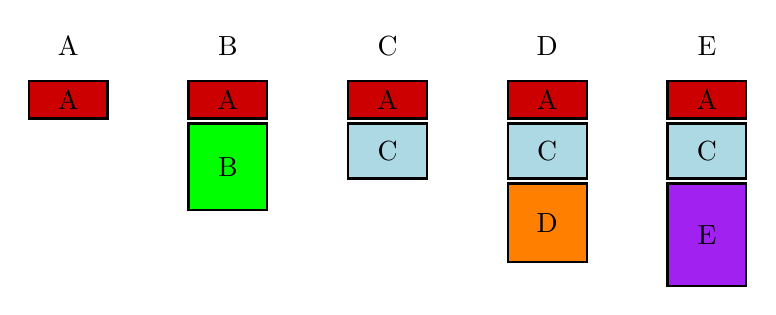
\begin{tikzpicture}[every node/.style={minimum width=1cm, rectangle,draw,thick}]
\node[draw=none] (a) at (0,0) {A};
\node[fill=red3,below=5pt of a] {A};

\node[right=1cm of a,draw=none] (b) {B};
\node[fill=red3,below=5pt of b] (b1) {A};
\node[fill=green,below=1pt of b1,minimum height=1.1cm] {B};

\node[right=1cm of b,draw=none] (c) {C};
\node[fill=red3,below=5pt of c] (c1) {A};
\node[fill=lightblue,below=1pt of c1,minimum height=.7cm] {C};

\node[right=1cm of c,draw=none] (d) {D};
\node[fill=red3,below=5pt of d] (d1) {A};
\node[fill=lightblue,below=1pt of d1,minimum height=.7cm] (d2) {C};
\node[fill=orange,below=1pt of d2,minimum height=1cm] {D};

\node[right=1cm of d,draw=none] (e) {E};
\node[fill=red3,below=5pt of e] (e1) {A};
\node[fill=lightblue,below=1pt of e1,minimum height=.7cm] (e2) {C};
\node[fill=purple,below=1pt of e2,minimum height=1.3cm] {E};
\end{tikzpicture}

\end{document}
